% Volumenelement in Kugelkoordinaten: Kantenlängen dr, r dtheta, r sin(theta) dphi
% Gemeinsamer Stil für alle Abbildungen (TikZ -> SVG, siehe figures/build.mjs).
%
% Farben sind Platzhalter ("Sentinels"): build.mjs ersetzt sie im SVG durch
% CSS-Variablen, damit die Abbildungen im hellen und dunklen Modus passen.
% Andere Farben (auch schwarz/weiß) bricht der Build mit Fehler ab.
%
%   fg    Linien, Beschriftung          -> --dark
%   mu    Hilfslinien, Achsen, Maße      -> --gray
%   acc   das eine Konzept der Abbildung -> --secondary (Lime/Oliv)
%   blue  zweite Größe, negative Ladung  -> --fig-blue
%   warm  dritte Größe, positive Ladung  -> --fig-warm
%   bg    Seitenhintergrund (Aussparen)  -> --light
%
% Kein \clip verwenden: pdftocairo macht daraus Clip-Gruppen, in denen exakt
% waagerechte/senkrechte Linien verschwinden. Berechnete Kurven schneidet
% gen/*.py selbst am Rahmen ab.
\documentclass[tikz,border=3pt]{standalone}
\usepackage{amsmath,amssymb,bm}
% Text serifenlos wie die Seite, Mathe in Computer Modern wie KaTeX
\renewcommand{\familydefault}{\sfdefault}
\usetikzlibrary{arrows.meta,calc,decorations.markings,patterns,3d,positioning,angles,quotes}

\definecolor{fg}{RGB}{1,2,3}
\definecolor{mu}{RGB}{4,5,6}
\definecolor{acc}{RGB}{7,8,9}
\definecolor{blue}{RGB}{10,11,12}
\definecolor{warm}{RGB}{13,14,15}
\definecolor{bg}{RGB}{16,17,18}

% Vektoren wie auf der Website (KaTeX \mathbf)
\newcommand{\vv}[1]{\mathbf{#1}}

\tikzset{
  every picture/.style={fg, line width=0.8pt, line cap=round, line join=round,
    >={Stealth[length=5.5pt,width=4.4pt]}},
  every node/.style={font=\small},
  % Linientypen
  main/.style={line width=0.9pt},
  thin/.style={line width=0.5pt},
  aux/.style={mu, line width=0.5pt, dash pattern=on 2.5pt off 2pt},
  axis/.style={mu, line width=0.6pt, ->},
  vec/.style={line width=1.1pt, ->},
  field/.style={line width=0.7pt, postaction={decorate},
    decoration={markings, mark=at position #1 with {\arrow{Stealth[length=4.5pt,width=3.6pt]}}}},
  field/.default=0.5,
  % Flächen
  soft/.style={fill=#1, fill opacity=0.14},
  soft/.default=acc,
  % Ladungen
  qpos/.style={circle, fill=warm, inner sep=0pt, minimum size=9pt,
    path picture={\draw[bg, line width=0.9pt] ($(path picture bounding box.center)+(-2pt,0)$) -- +(4pt,0)
      ($(path picture bounding box.center)+(0,-2pt)$) -- +(0,4pt);}},
  qneg/.style={circle, fill=blue, inner sep=0pt, minimum size=9pt,
    path picture={\draw[bg, line width=0.9pt] ($(path picture bounding box.center)+(-2pt,0)$) -- +(4pt,0);}},
  dot/.style={circle, fill=fg, inner sep=0pt, minimum size=3pt},
  % Beschriftung mit Aussparung, damit Linien den Text nicht kreuzen
  lbl/.style={fill=bg, inner sep=1.5pt},
  % Icons: kräftigere Linien, keine Schrift
  icon/.style={line width=1.6pt, >={Stealth[length=6pt,width=5pt]}},
}

\begin{document}
% Projektion: x nach vorn-links, y nach rechts, z nach oben. Blickrichtung und (theta, phi)
% so gewählt, dass r-, theta- und phi-Kanten auf dem Bildschirm >= 55 Grad auseinanderliegen.
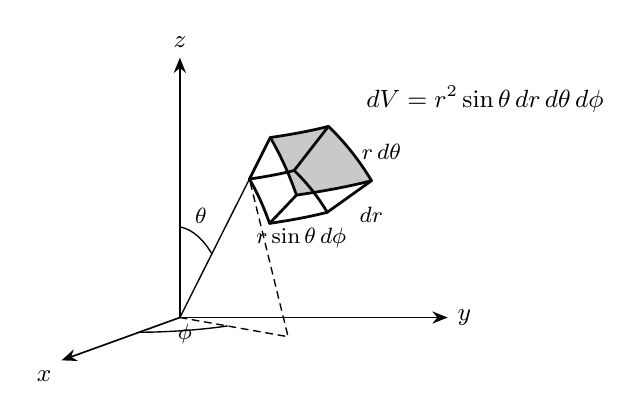
\begin{tikzpicture}[declare function={sx(\R,\T,\P)=\R*sin(\T)*cos(\P); sy(\R,\T,\P)=\R*sin(\T)*sin(\P); sz(\R,\T)=\R*cos(\T);},
  x={(-0.47cm,-0.17cm)}, y={(1cm,0cm)}, z={(0cm,1cm)}]
  \def\r{2.5} \def\dr{0.75}
  \def\th{40} \def\dth{16}
  \def\ph{55} \def\dph{25}
  % Punkt in Kugelkoordinaten
  \newcommand{\sph}[3]{({(#1)*sin(#2)*cos(#3)},{(#1)*sin(#2)*sin(#3)},{(#1)*cos(#2)})}
  % Achsen
  \draw[axis] (0,0,0) -- (3.2,0,0) node[anchor=north east, text=fg] {$x$};
  \draw[axis] (0,0,0) -- (0,3.4,0) node[anchor=west, text=fg] {$y$};
  \draw[axis] (0,0,0) -- (0,0,3.3) node[anchor=south, text=fg] {$z$};
  % Hilfslinien: Radiusvektor, Projektion in die xy-Ebene
  \draw[thin] (0,0,0) -- \sph{\r}{\th}{\ph};
  \draw[aux] (0,0,0) -- \sph{\r}{90}{\ph} -- \sph{\r}{\th}{\ph};
  % Winkel theta (in der Ebene phi = const) und phi (in der xy-Ebene)
  \draw[mu, thin, domain=0:\th, samples=30, variable=\t] plot ({sx(1.15,\t,\ph)},{sy(1.15,\t,\ph)},{sz(1.15,\t)});
  \node[text=mu, font=\footnotesize] at \sph{1.42}{\th/2}{\ph} {$\theta$};
  \draw[mu, thin, domain=0:\ph, samples=30, variable=\t] plot ({sx(1.1,90,\t)},{sy(1.1,90,\t)},{sz(1.1,90)});
  \node[text=mu, font=\footnotesize] at \sph{1.4}{90}{\ph/2} {$\phi$};
  % Volumenelement: Außenfläche (r+dr) getönt
  \fill[acc, fill opacity=0.22]
    plot[domain=\th:\th+\dth, samples=12, variable=\t] ({sx(\r+\dr,\t,\ph)},{sy(\r+\dr,\t,\ph)},{sz(\r+\dr,\t)})
    -- plot[domain=\ph:\ph+\dph, samples=12, variable=\t] ({sx(\r+\dr,\th+\dth,\t)},{sy(\r+\dr,\th+\dth,\t)},{sz(\r+\dr,\th+\dth)})
    -- plot[domain=\th+\dth:\th, samples=12, variable=\t] ({sx(\r+\dr,\t,\ph+\dph)},{sy(\r+\dr,\t,\ph+\dph)},{sz(\r+\dr,\t)})
    -- plot[domain=\ph+\dph:\ph, samples=12, variable=\t] ({sx(\r+\dr,\th,\t)},{sy(\r+\dr,\th,\t)},{sz(\r+\dr,\th)}) -- cycle;
  \begin{scope}[acc, line width=1pt]
    \foreach \R in {\r,\r+\dr} {
      \draw plot[domain=\th:\th+\dth, samples=12, variable=\t] ({sx(\R,\t,\ph)},{sy(\R,\t,\ph)},{sz(\R,\t)});
      \draw plot[domain=\th:\th+\dth, samples=12, variable=\t] ({sx(\R,\t,\ph+\dph)},{sy(\R,\t,\ph+\dph)},{sz(\R,\t)});
      \draw plot[domain=\ph:\ph+\dph, samples=12, variable=\t] ({sx(\R,\th,\t)},{sy(\R,\th,\t)},{sz(\R,\th)});
      \draw plot[domain=\ph:\ph+\dph, samples=12, variable=\t] ({sx(\R,\th+\dth,\t)},{sy(\R,\th+\dth,\t)},{sz(\R,\th+\dth)});
    }
    \foreach \T/\P in {\th/\ph, \th+\dth/\ph, \th/\ph+\dph, \th+\dth/\ph+\dph}
      \draw \sph{\r}{\T}{\P} -- \sph{\r+\dr}{\T}{\P};
  \end{scope}
  % Kantenbeschriftung (Kanten an der vorderen rechten Ecke theta+dtheta, phi+dphi)
  \node[anchor=north west, font=\footnotesize] at \sph{\r+\dr/2}{\th+\dth}{\ph+\dph} {$dr$};
  \node[anchor=west, font=\footnotesize] at \sph{\r+\dr}{\th+\dth/2}{\ph+\dph} {$r\,d\theta$};
  \node[anchor=north, font=\footnotesize] at \sph{\r}{\th+\dth}{\ph+\dph/2} {$r\sin\theta\,d\phi$};
  \path \sph{\r+\dr}{\th}{\ph+\dph} coordinate (T);
  \node[anchor=south west] at ($(T)+(0,0.35,0.05)$) {$dV=r^2\sin\theta\,dr\,d\theta\,d\phi$};
\end{tikzpicture}
\end{document}
